\section{Conclusion}
\label{sec:conclude}
\begin{figure}
  \centering
  {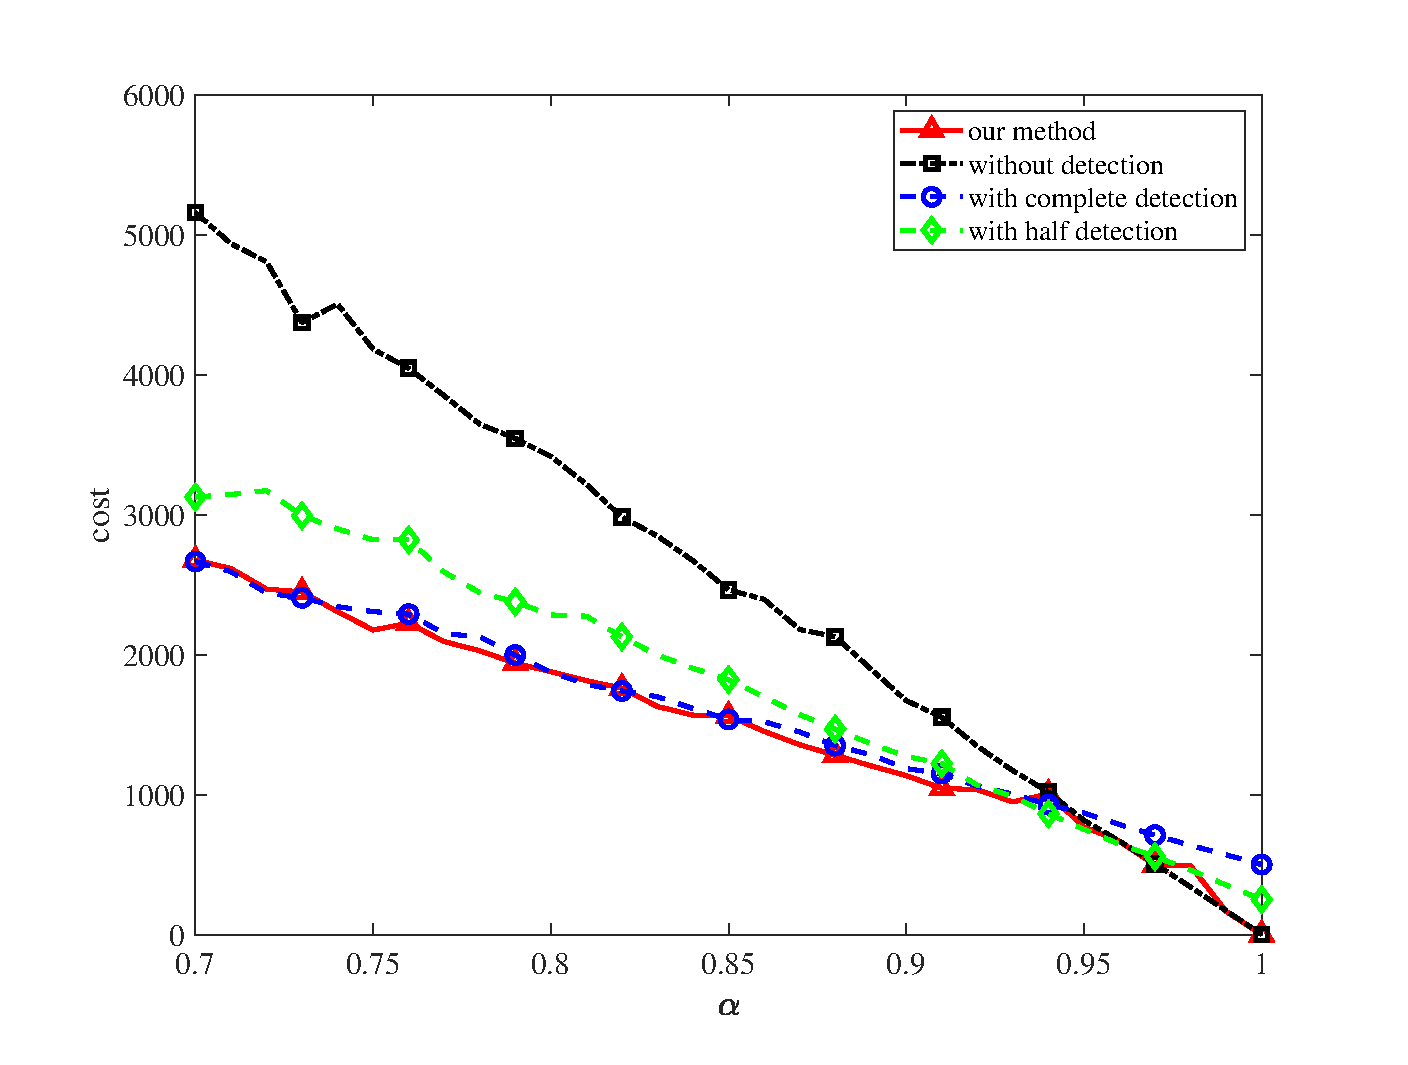
\includegraphics[width=0.45\textwidth]{fig/cost_vs_alpha.eps}}
     \caption{Total cost $J$ vs. $\alpha$.}
     \label{fig:cost_alpha}
\end{figure}
In this paper, we have analytically investigated
the state transition of nodes in the opportunistic networks.
The ordinary differential equation models have been constructed to
capture the message dissemination with complete detection,
which can suppress the increment of selfish node number.
To achieve the tradeoff the reward and the detection cost
in the message lifetime,
we propose the optimal solution of the selfish node detection
based on the Pontryagin's maximum principle.
The soundness of the models and the accuracy of the analysis
have been verified via extensive simulation.

Through the proposed method,
it is clear that the optimal solution of selfish node detection
can be obtained
when the change rate of becoming selfish is constant.
%the strategy of the relay nodes is stable, i.e.,
%the unit paid reward is constant.
Inspired by this,
we will study effective methods
to minimize the combination of
the total paid reward and the detection cost
when the change rate of becoming selfish
and the unit paid reward
are variable with time in the future.
